\documentclass[10 pt,usenames,dvipsnames, oneside]{article}
\usepackage{../../modelo-fracoes}
\graphicspath{{../../../Figuras/licao01/}}


\begin{document}

\begin{center}
  \begin{minipage}[l]{3cm}

\includegraphics[width=2cm]{../../../Figuras/logo}       
\end{minipage}\hfill
\begin{minipage}[r]{.8\textwidth}
 {\Large \scshape Atividade: Discos de frações, nome e comparação}  
\end{minipage}
\end{center}
\vspace{.2cm}

\ifdefined\prof
\begin{goals}
\begin{enumerate}

 \item Distinguir e nomear frações unitárias a partir de suas representações em modelos circulares.
\item  Comparar frações unitárias a partir de suas representações em modelos circulares.

\end{enumerate}
\tcblower

\begin{itemize}
\item    Esta atividade é planejada para ser desenvolvida a partir de material concreto baseado em modelos circulares. Mais especificamente com um material conhecido como ``Círculos de Frações''. Para aplicá-la, é necessário reproduzir esse material, que está disponível nas páginas para reprodução.
\item Sendo um material concreto, os círculos de frações têm o papel de auxiliar na visualização da representação das frações, mais especificamente, das frações unitárias.
\item Recomenda-se que esta atividade seja desenvolvida em grupos de 3 a 5 alunos. No entanto, cada aluno deve ter o seu próprio material (Círculos de Frações) para realizar a atividade.
\item Durante a discussão, os alunos devem ser estimulados a explicar as suas escolhas. O uso de cores vai fazer parte da comunicação, no entanto a justificativa e raciocínio devem estar apoiados no conceito de fração.
 \item Na versão utilizada nesta atividade, o círculo corresponde à unidade, ou seja, ao 1 e os setores circulares, diferenciados por cores, correspondem às frações unitárias um meio, um terço, um quarto, um sexto, um sétimo, um oitavo, um nono e um décimo.
    \item Refira-se ao círculo na cor preta como círculo ou unidade, e não como todo ou inteiro. Refira-se a cada setor circular como fração do círculo, parte do círculo ou, simplesmente, peça da cor x.
    \item Antes de solicitar aos alunos que realizem a atividade, explore o material ressaltando especialmente o fato de que, reunidas, as peças de uma mesma cor determinam um círculo congruente ao preto.
    \item Ainda antes de solicitar aos alunos que realizem a atividade, explore também o material com perguntas dirigidas a toda a turma como as seguintes: ``Quantas peças azuis cobrem o círculo preto?'' ou ``Quantas peças verdes cobrem o círculo preto?'', sugerindo que as peças coloridas podem ser consideradas frações do círculo preto.
    \item Faça uso do material concreto para ilustrar e explicar a resposta de cada item e incentive os seus alunos a fazerem o mesmo.
    \item Espera-se que a explicação para as respostas, nos oito primeiros itens desta questão, seja a partir da contagem dos setores circulares correspondentes às frações envolvidas. Assim, por exemplo, a resposta do item b) pode ser justificada pelo fato de que são necessários 4 partes de círculo na cor vermelha para compor um círculo preto.
    \item Já para os cinco itens que tratam da comparação, espera-se que os alunos identifiquem os setores que representam as frações envolvidas e procedam a comparação pela sobreposição das peças correspondentes. Assim, por exemplo, a resposta do item l) pode ser justificada pela sobreposição das peças das cores verde e amarelo.
    \item Aproveite a correção desses últimos itens para explorar, a partir dos Círculos de Frações, a relação entre a quantidade de peças de cada cor e o tamanho das peças, ou seja, a relação inversa entre a quantidade de partes em que círculo (unidade) está dividido e o tamanho de cada parte.
    \item Os Círculos de Frações podem ser utilizados para trabalhar outros conceitos e assuntos além de frações unitárias, tais como: frações em geral, comparação de frações e operações com frações (adição e subtração). 
    \end{itemize}


\end{goals}

\bigskip
\begin{center}
{\large \scshape Atividade}
\end{center}
\fi

Você receberá do seu professor círculos como os que seguem, todos de mesmo tamanho. 

\begin{center}

 \begin{tabular}{ccccccccc}

 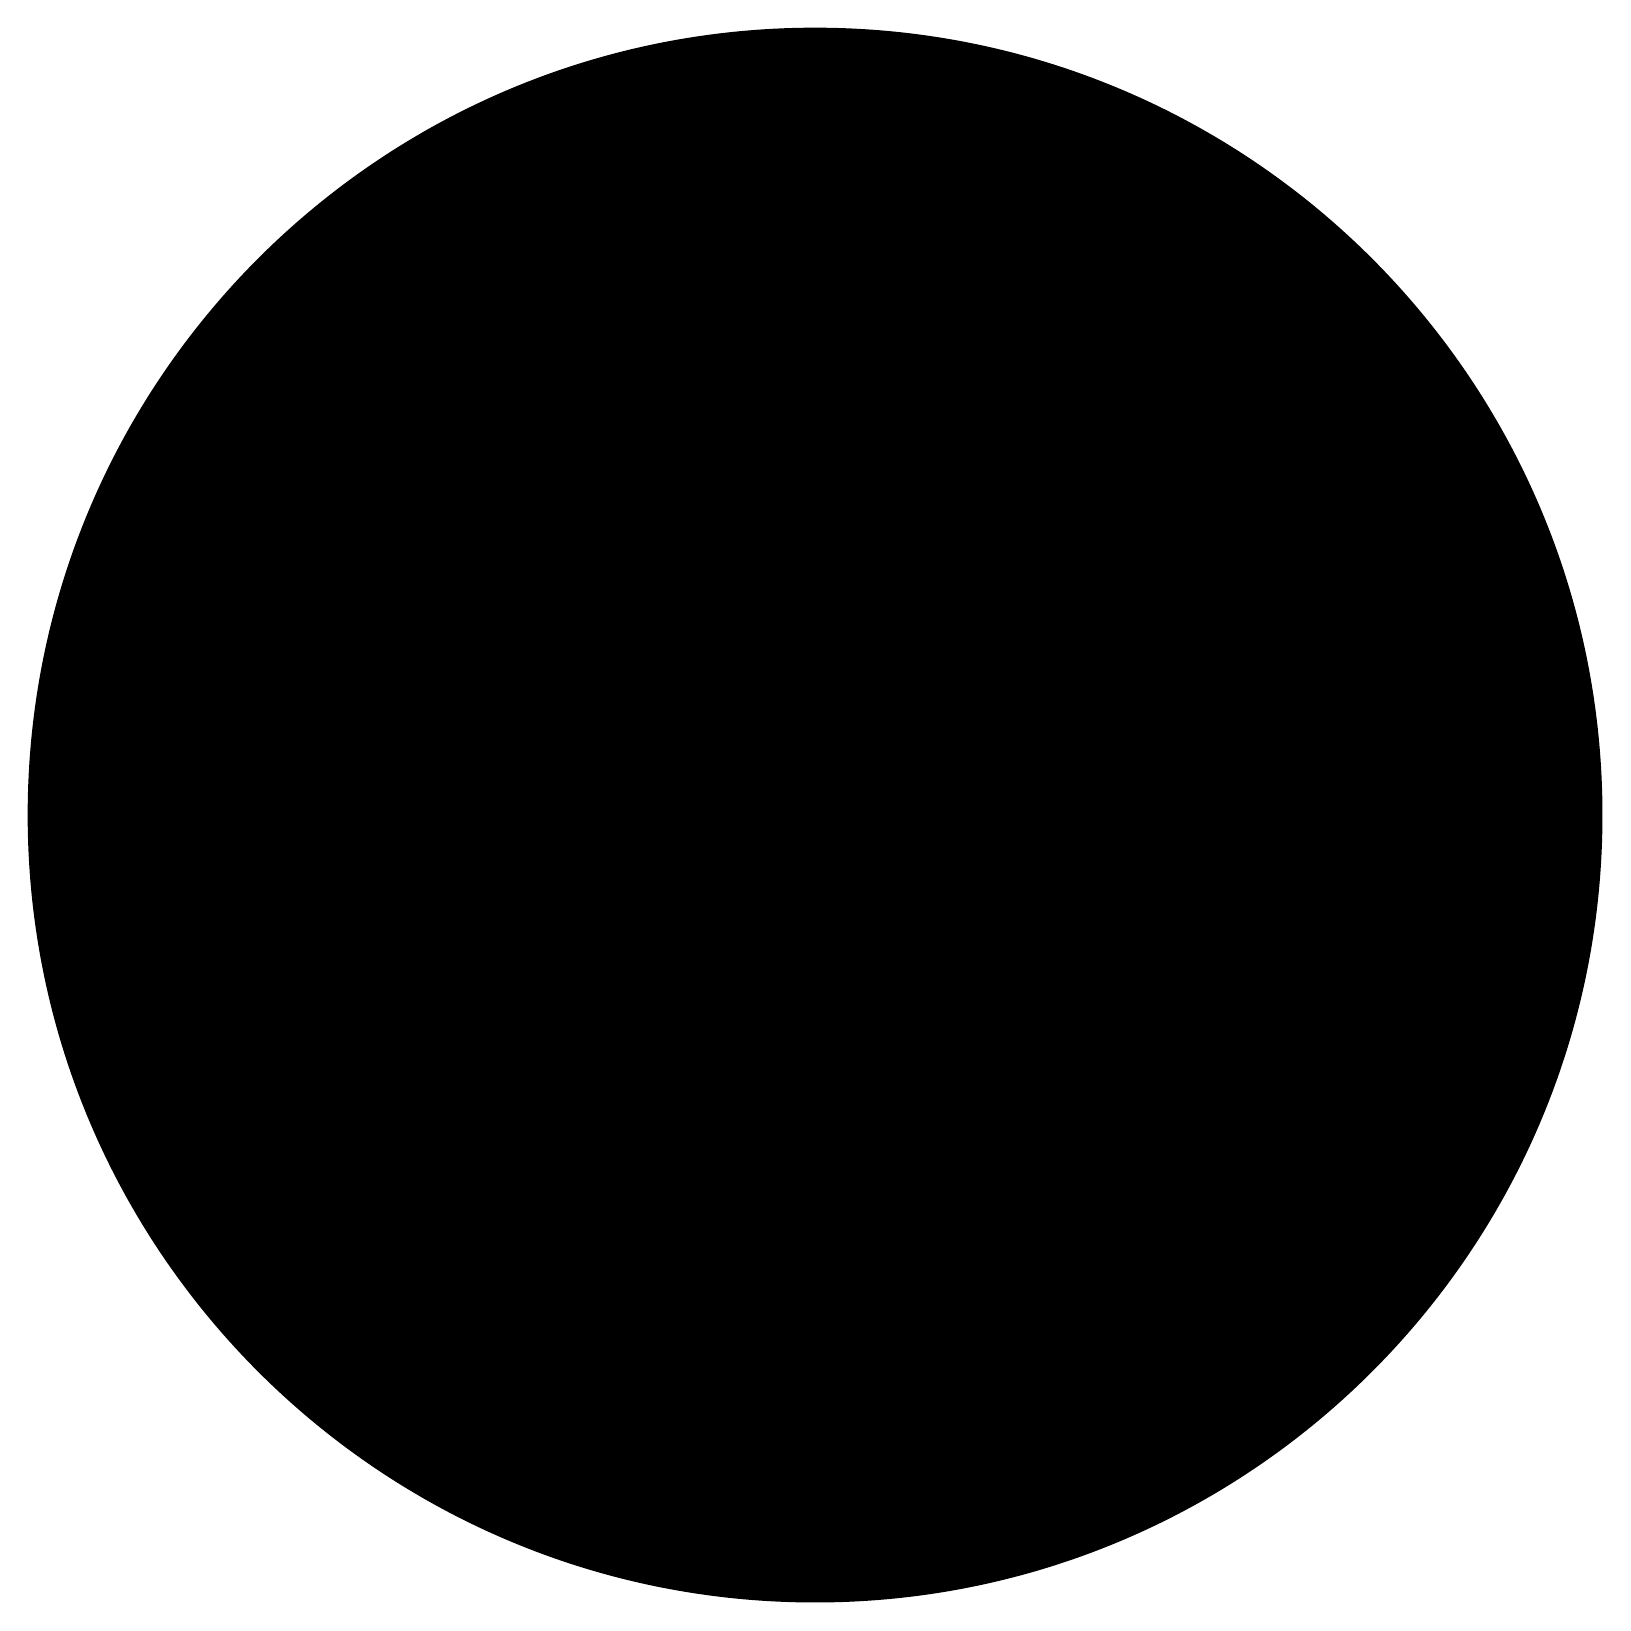
\begin{tikzpicture}
\fill[black] (0,0) circle (10);
 \end{tikzpicture}
& \parbox[t][.6cm][c]{1cm}{ }\quad&
 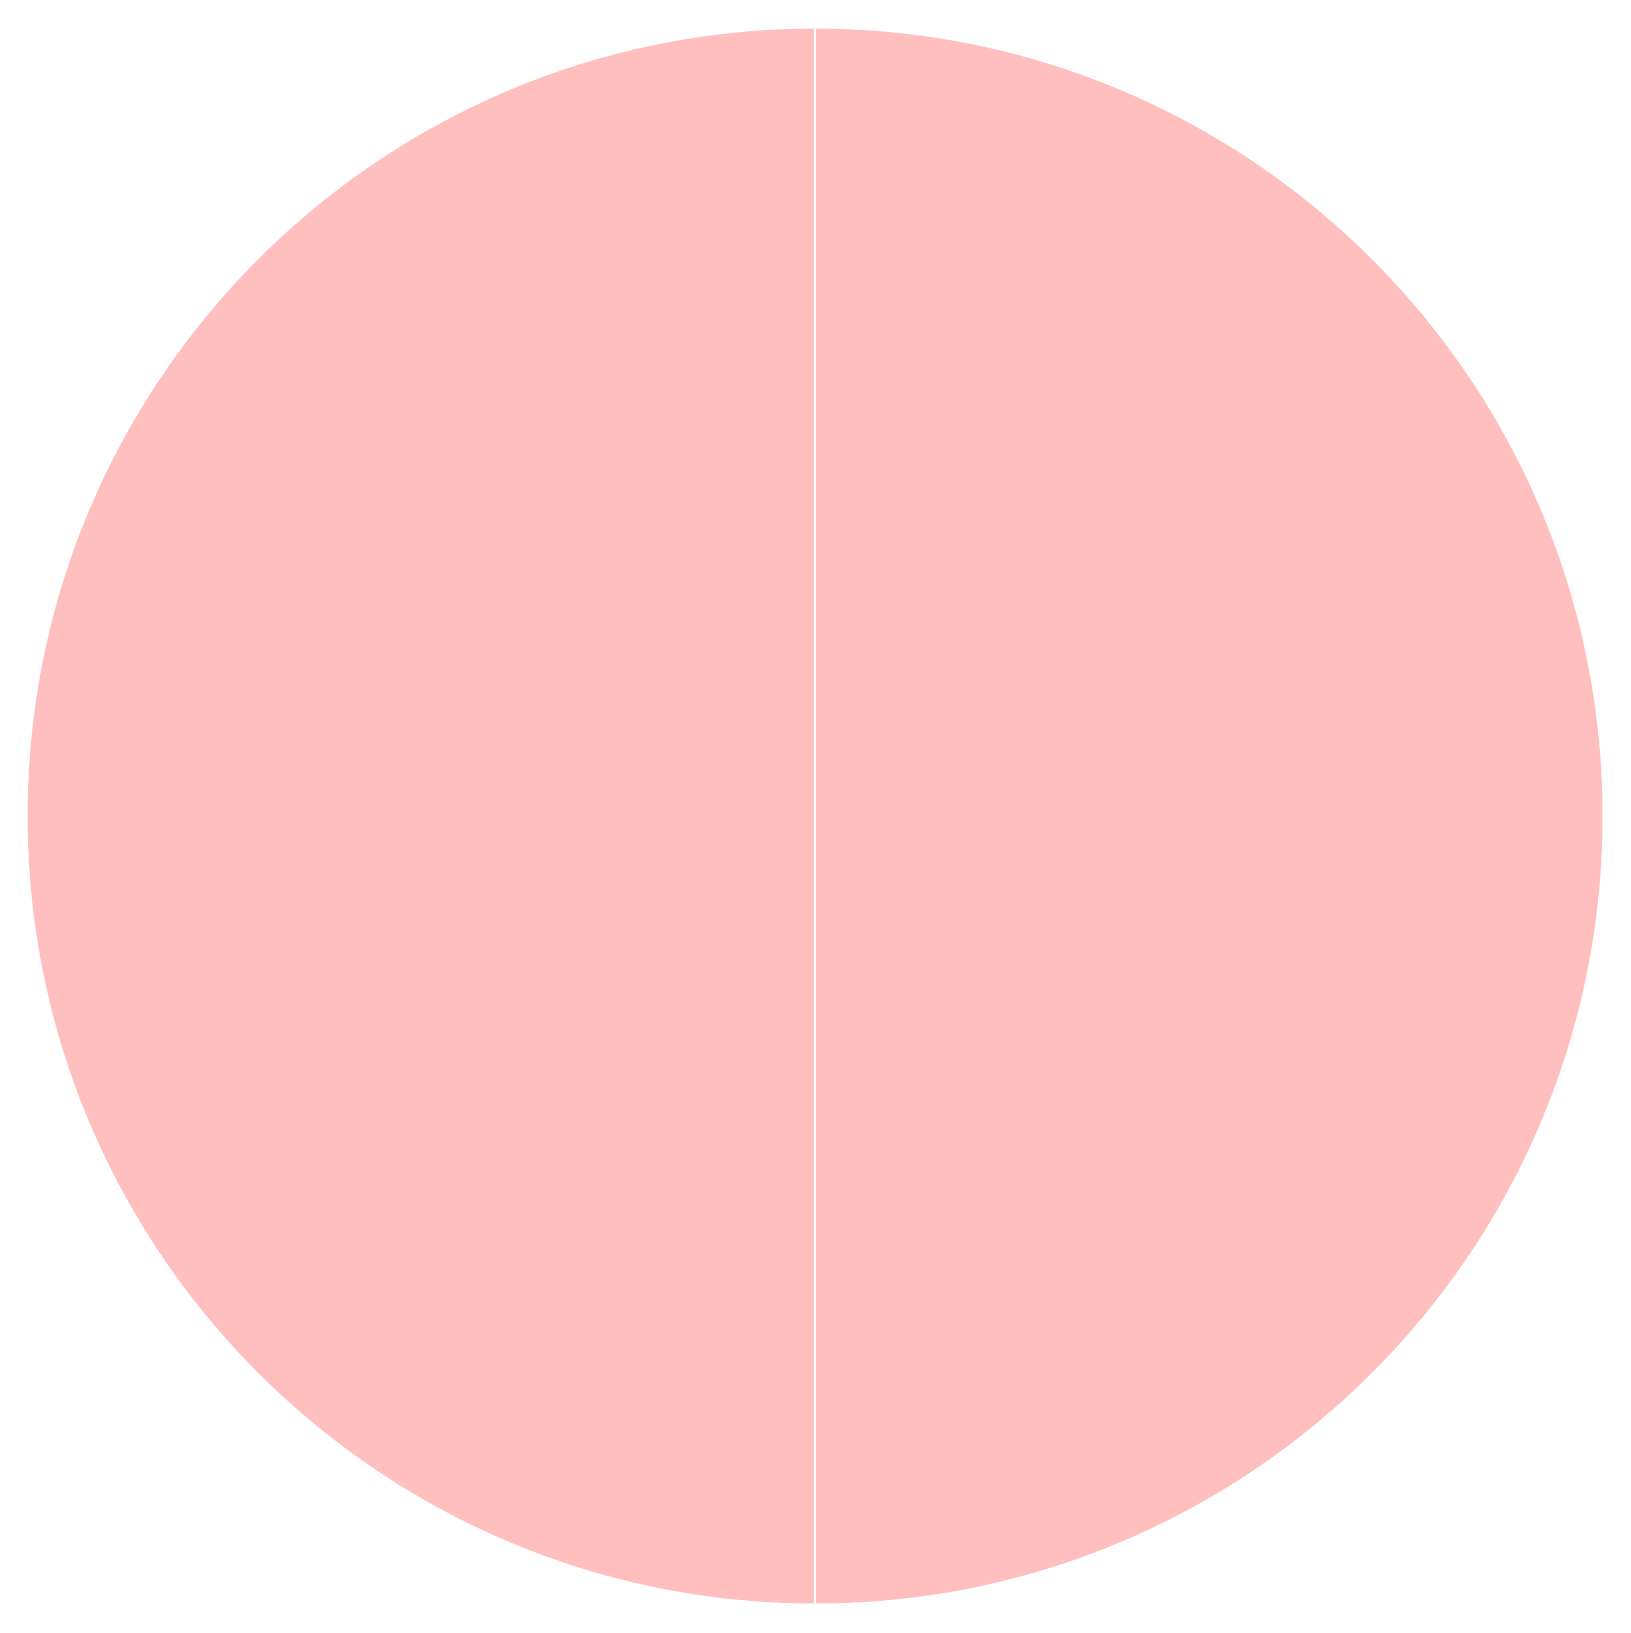
\begin{tikzpicture}
\fill[pink] (0,0) circle (10);
\draw[line width =.25mm, white] (-90:10) -- (90:10);
\end{tikzpicture}
& \quad&
 \begin{tikzpicture}
\fill[common] (0,0) circle (10);
\foreach \x in {30,150,270} \draw[line width =.25mm, white] (0,0)--(\x:10);
\end{tikzpicture}
& \quad&
 \begin{tikzpicture}
\fill[attention] (0,0) circle (10);
\foreach \x in {0,90} \draw[line width =.25mm, white] (\x:-10)--(\x:10);
\end{tikzpicture}
& \quad&
 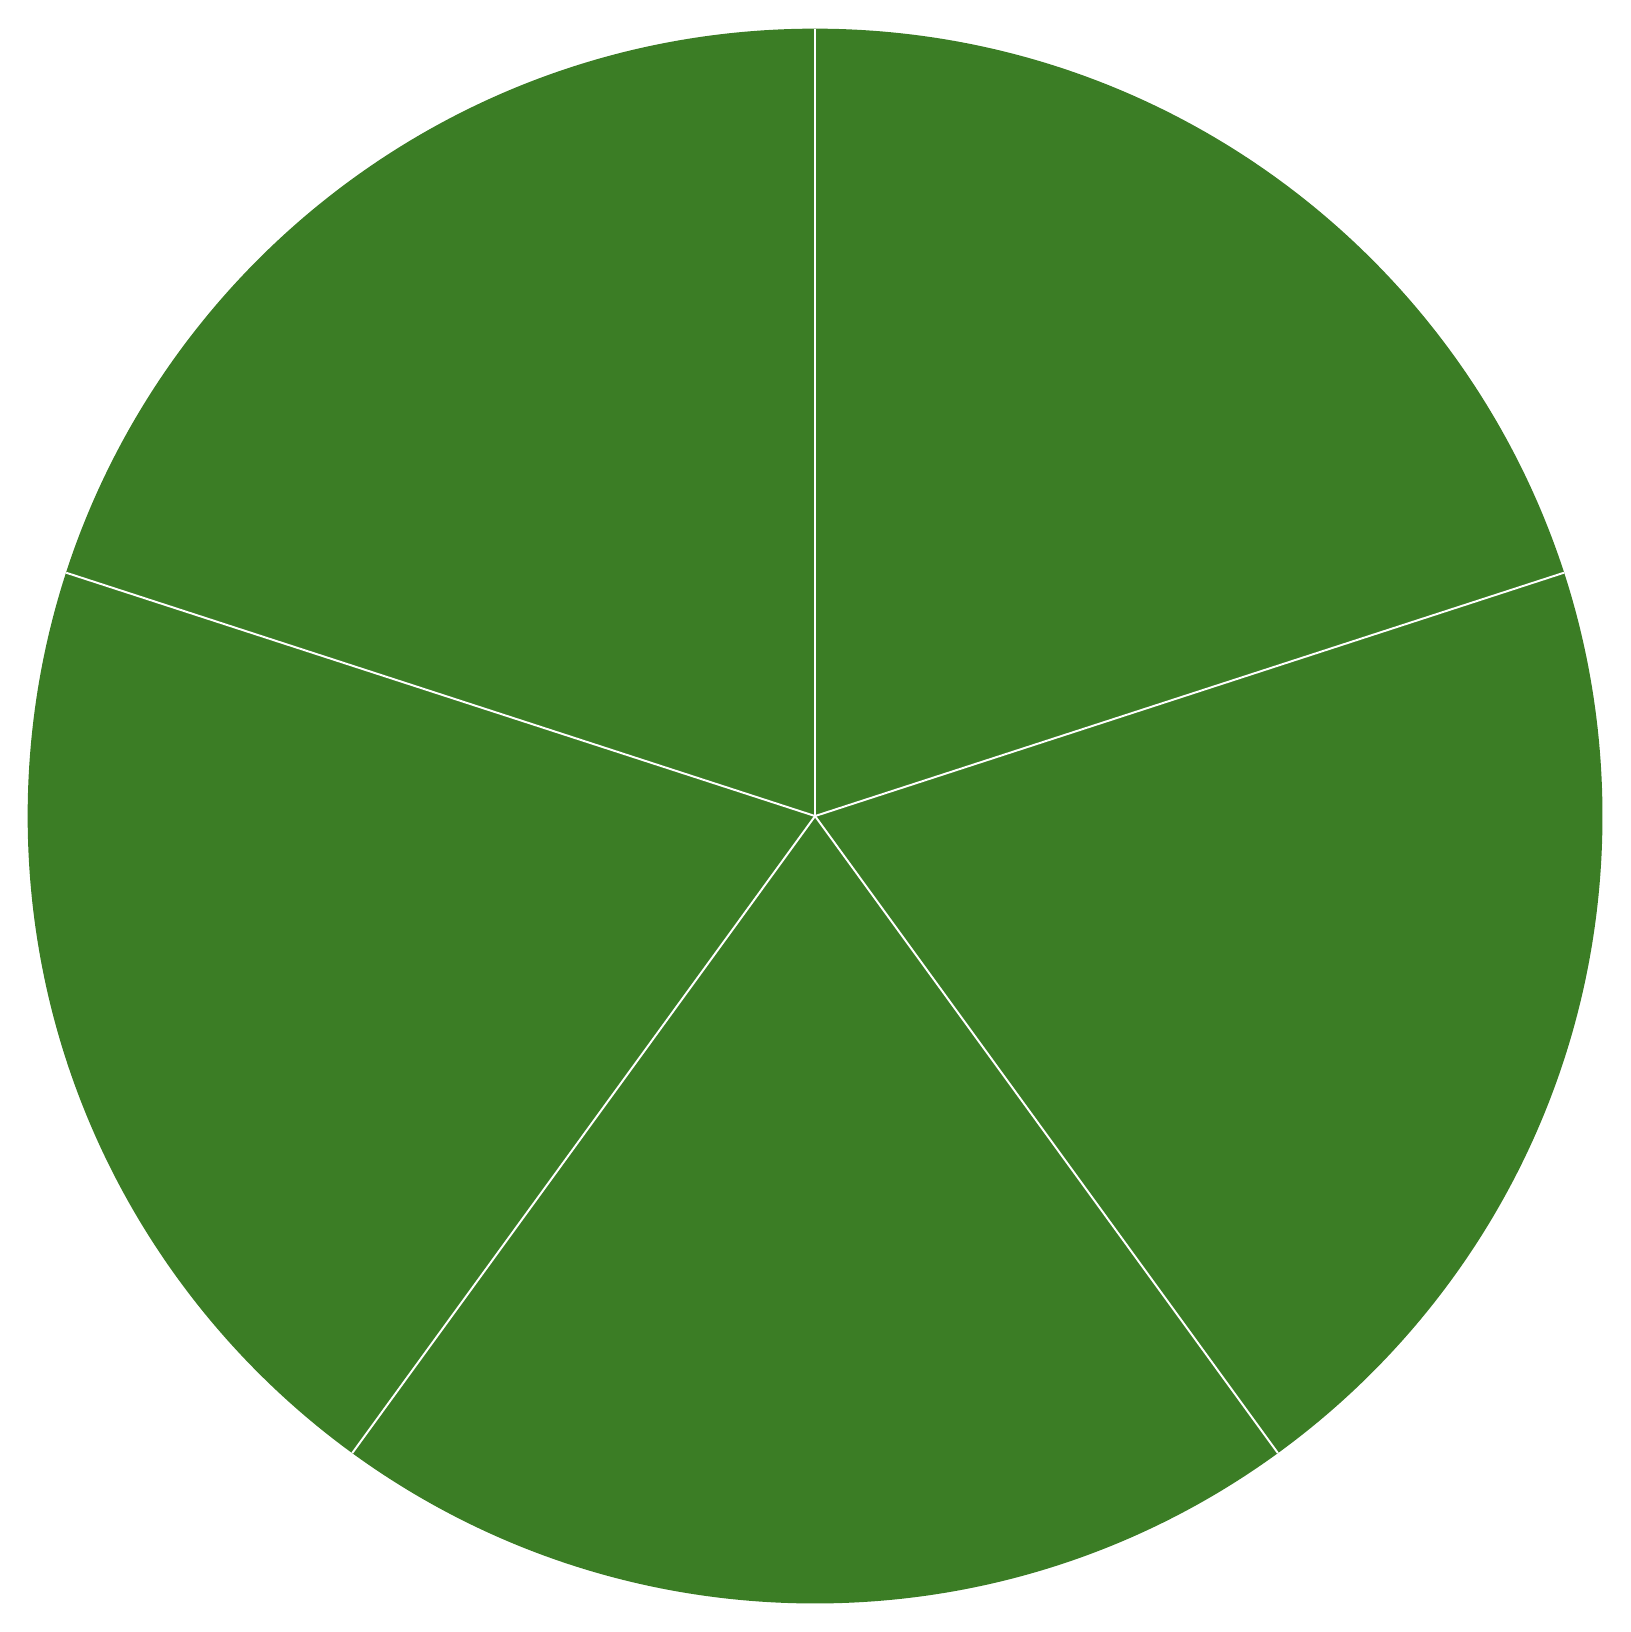
\begin{tikzpicture}
\fill[OliveGreen] (0,0) circle (10);
\foreach \x in {18,90,...,360} \draw[line width =.25mm, white] (0,0)--(\x:10);
\end{tikzpicture}\\
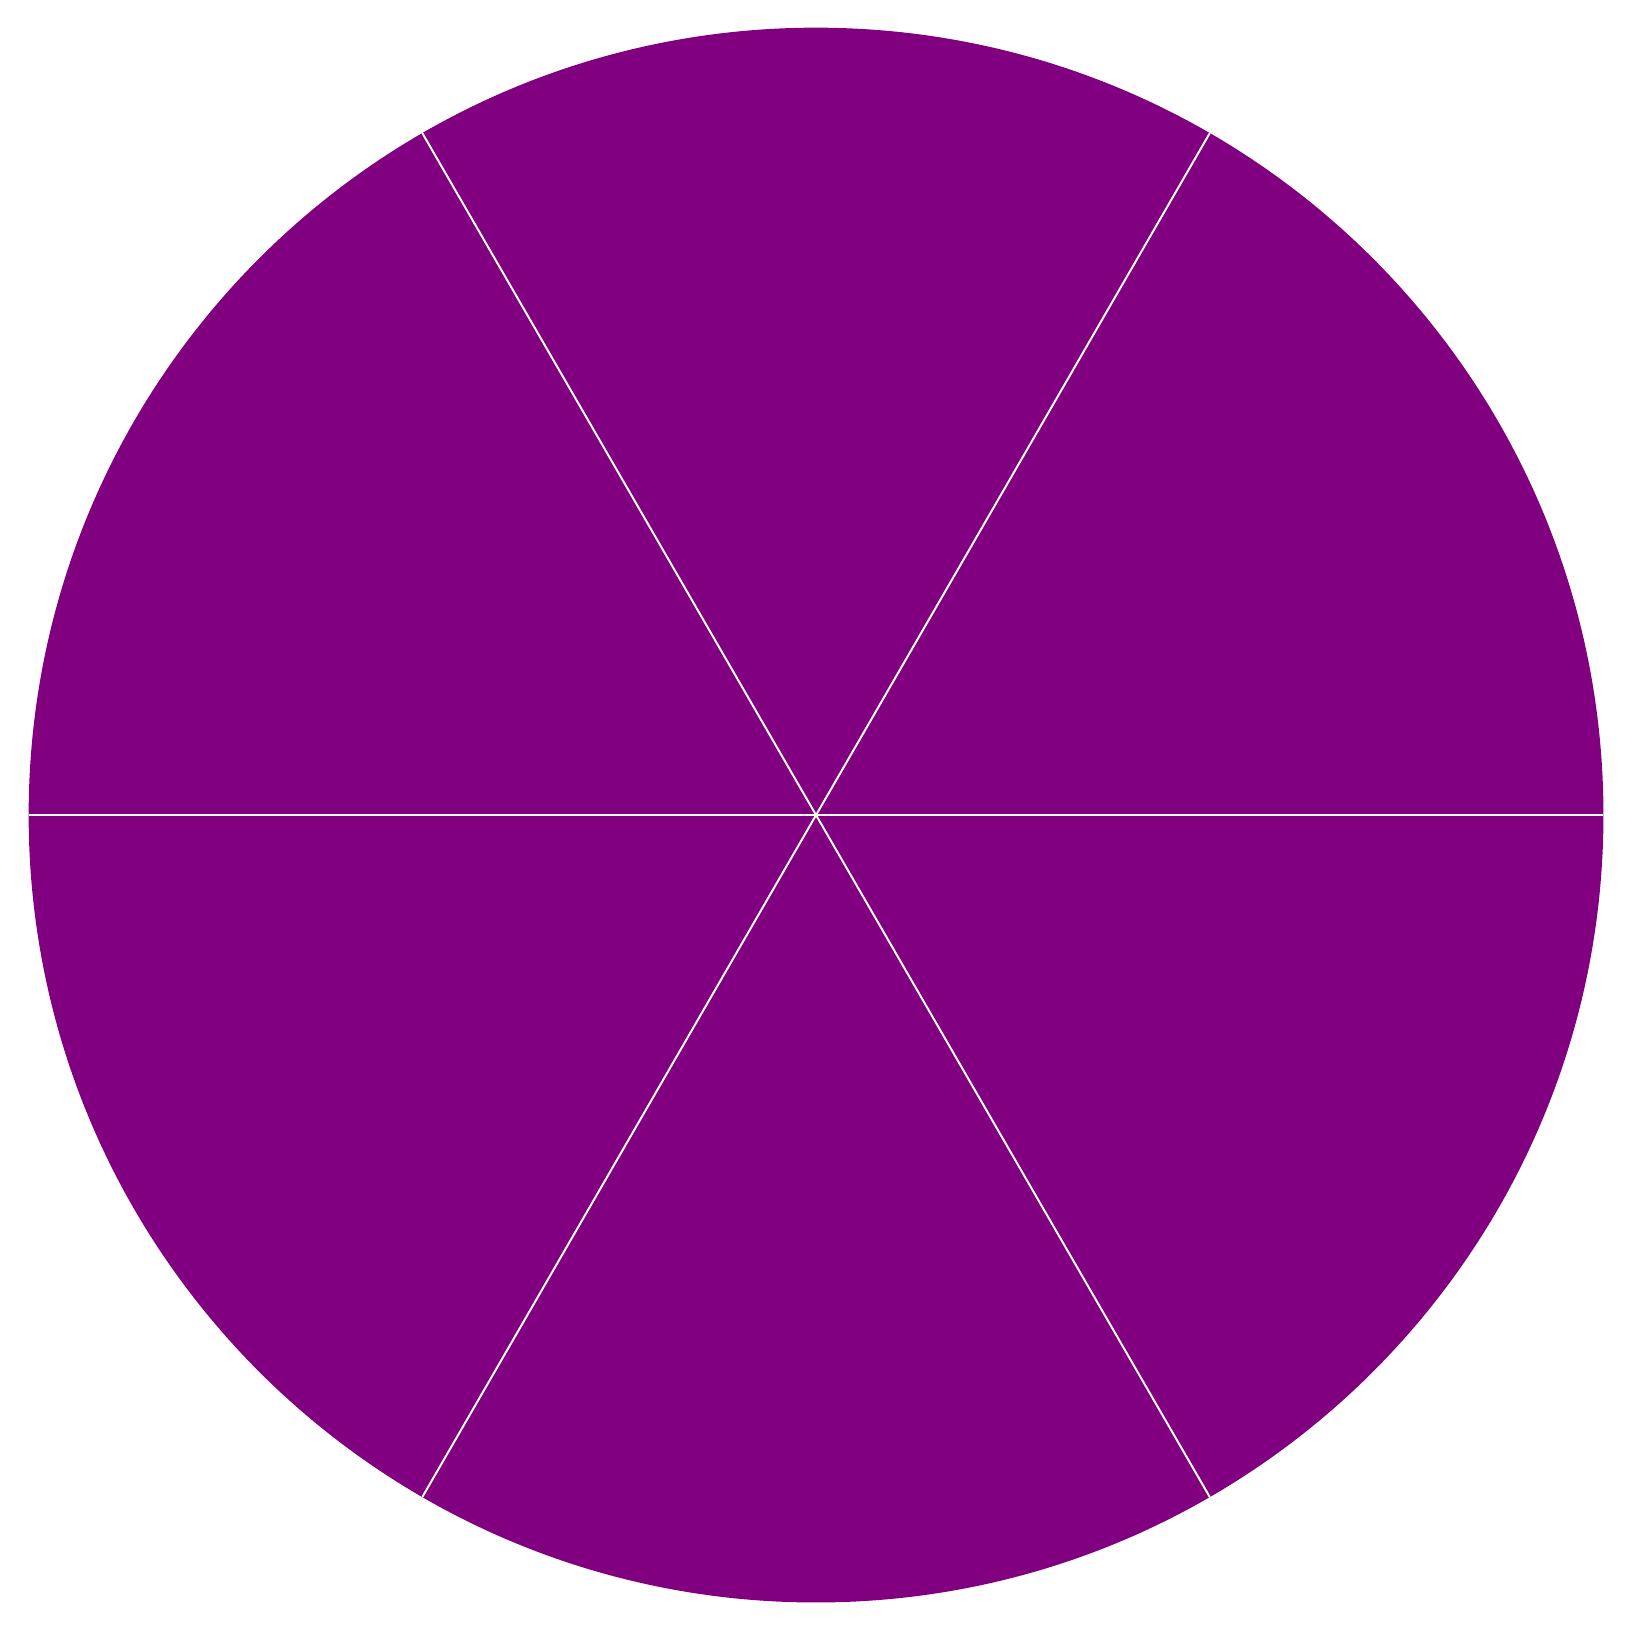
\begin{tikzpicture}
\fill[Purple] (0,0) circle (10);
\foreach \x in {0,60,...,360} \draw[line width =.25mm, white] (0,0)--(\x:10);
\end{tikzpicture}
& \parbox[t][.6cm][c]{1cm}{ }\quad&
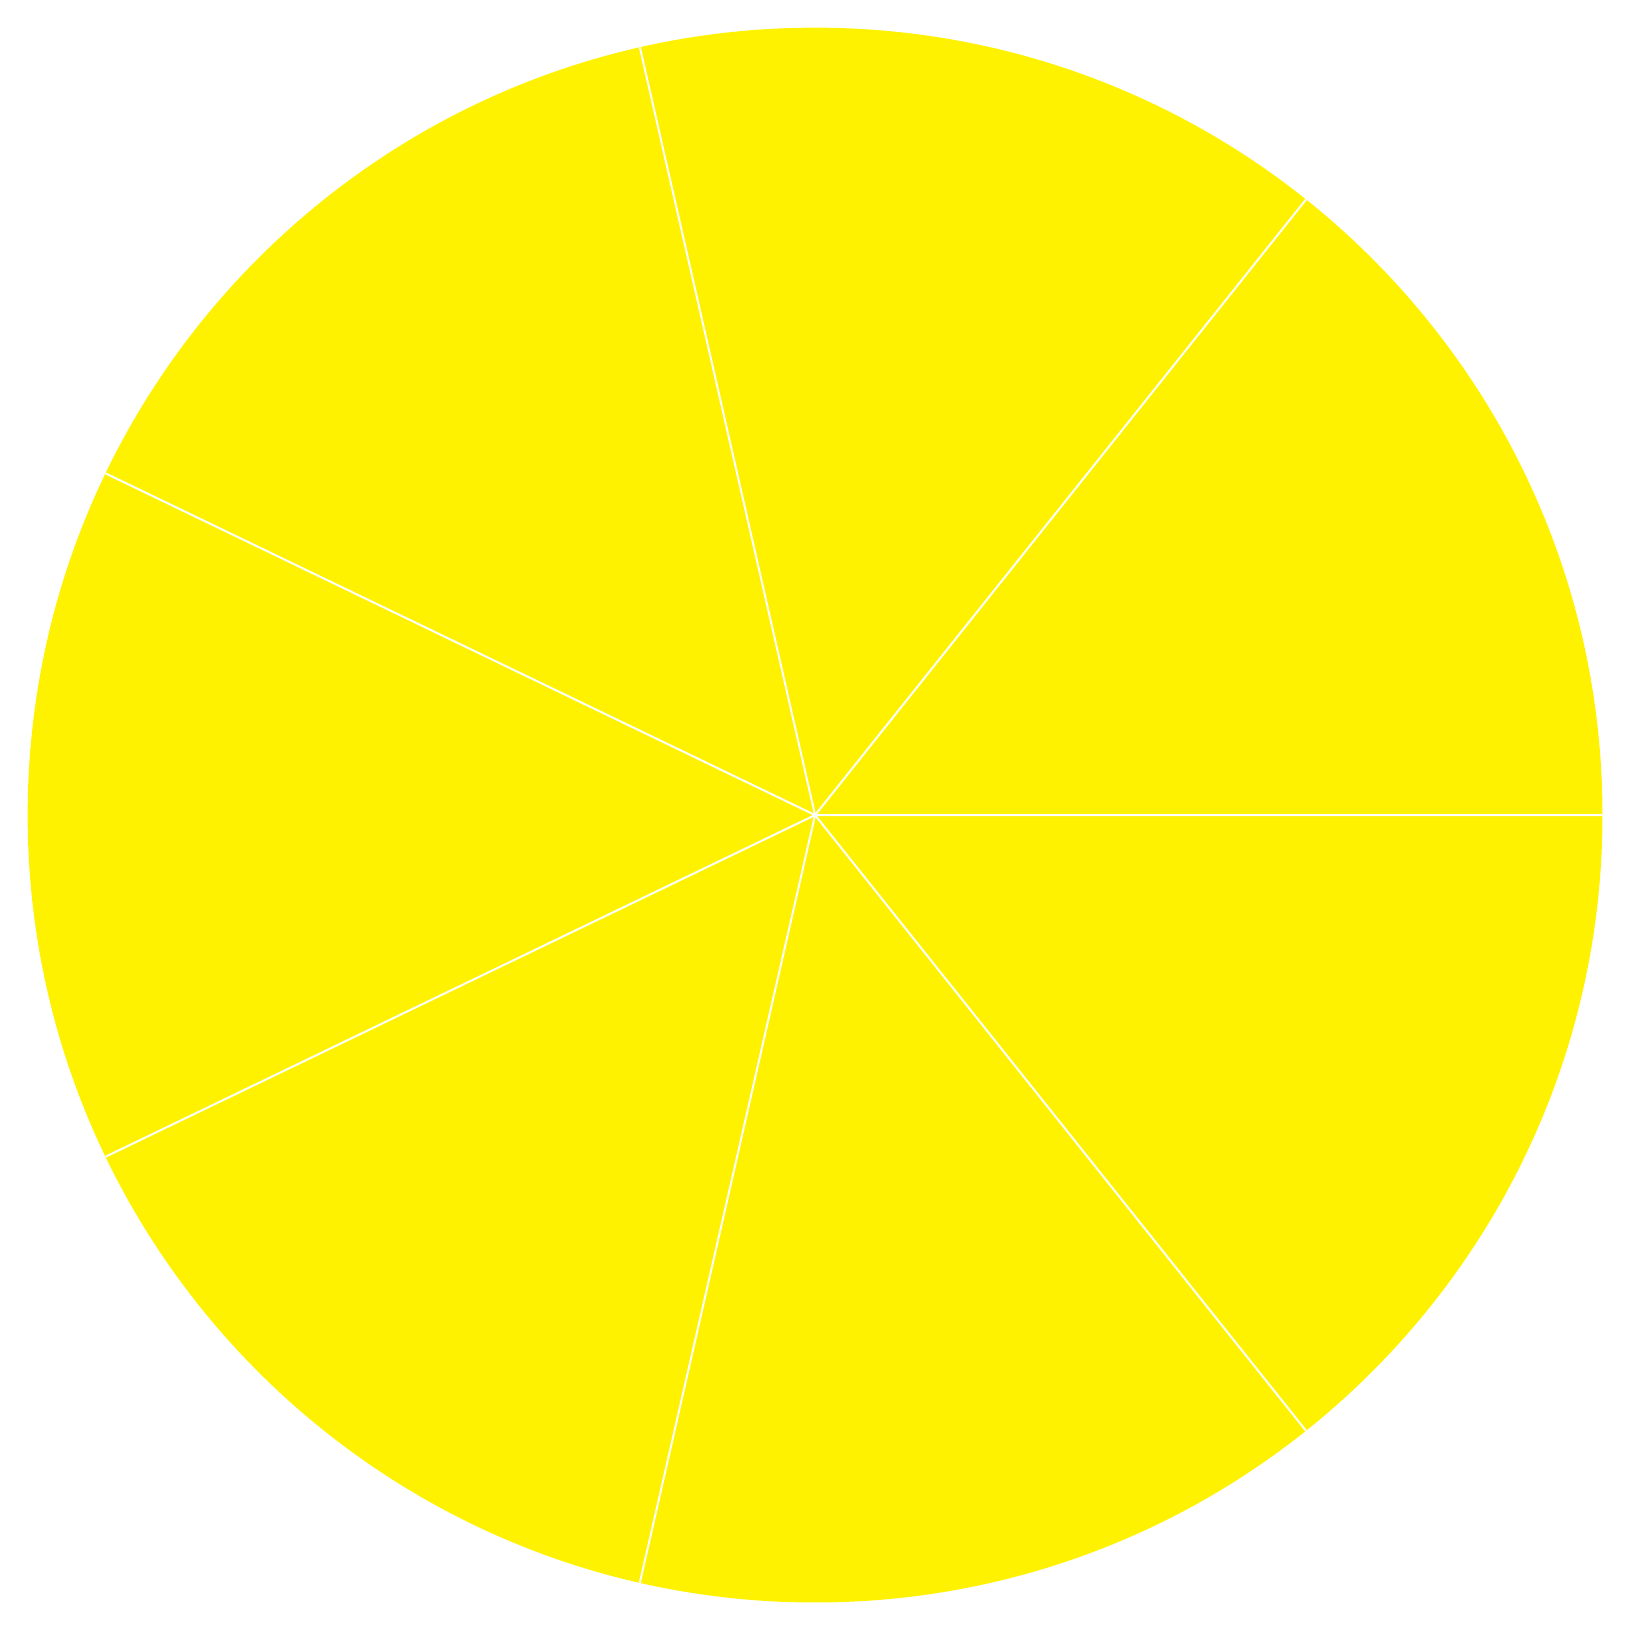
\begin{tikzpicture}
\fill[yellow] (0,0) circle (10);
\foreach \x in {0,51.428,...,360} \draw[line width =.25mm, white] (0,0)--(\x:10);
\end{tikzpicture}
&\parbox[t][.6cm][c]{1cm}{ }&
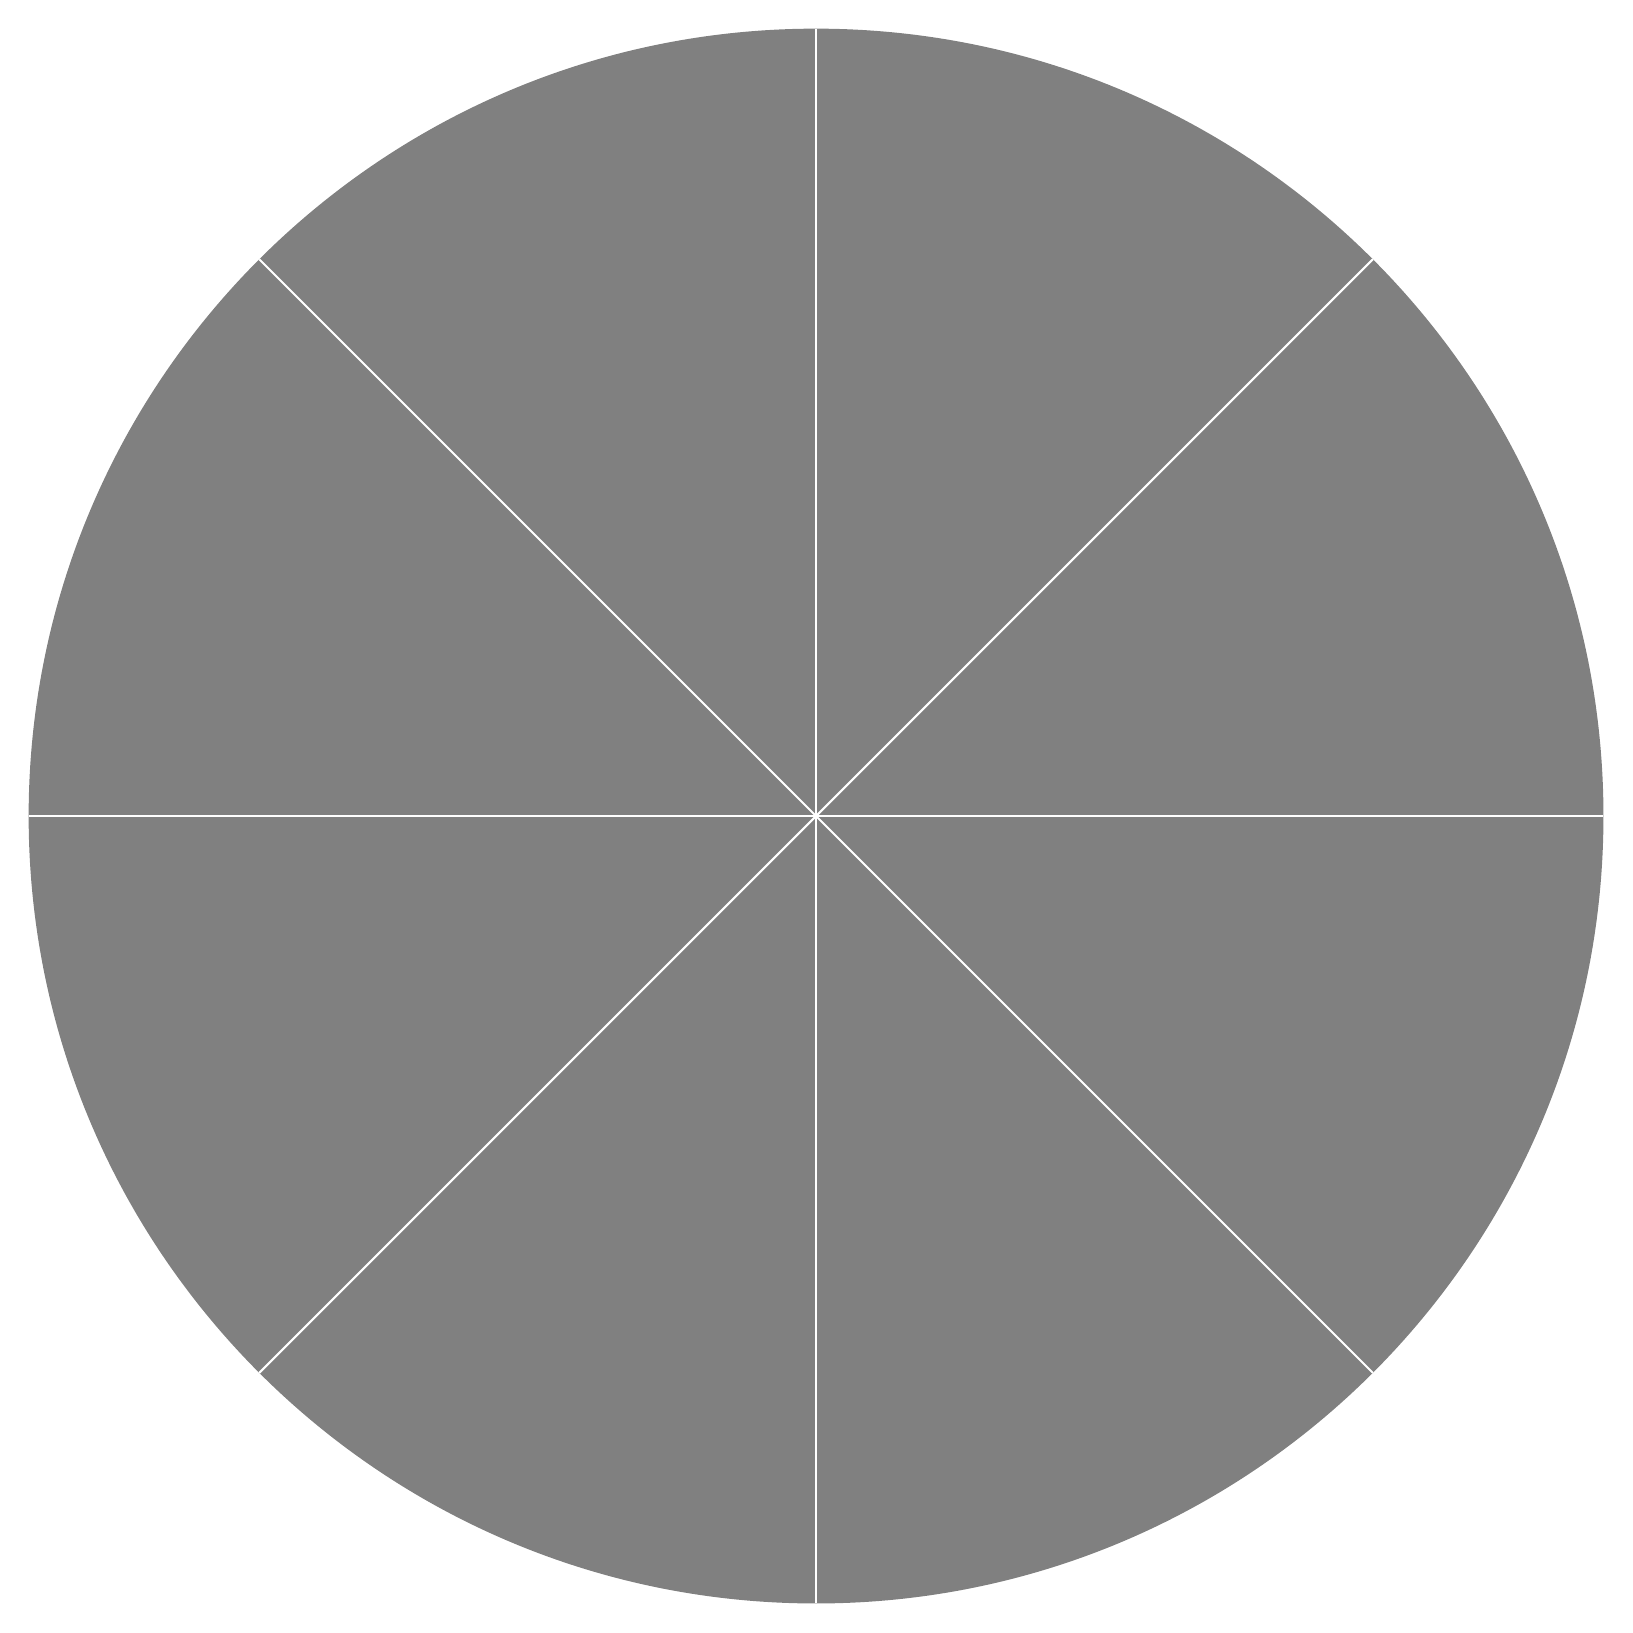
\begin{tikzpicture}
\fill[gray] (0,0) circle (10);
\foreach \x in {0,45,...,360} \draw[line width =.25mm, white] (0,0)--(\x:10);
\end{tikzpicture}
& \quad&
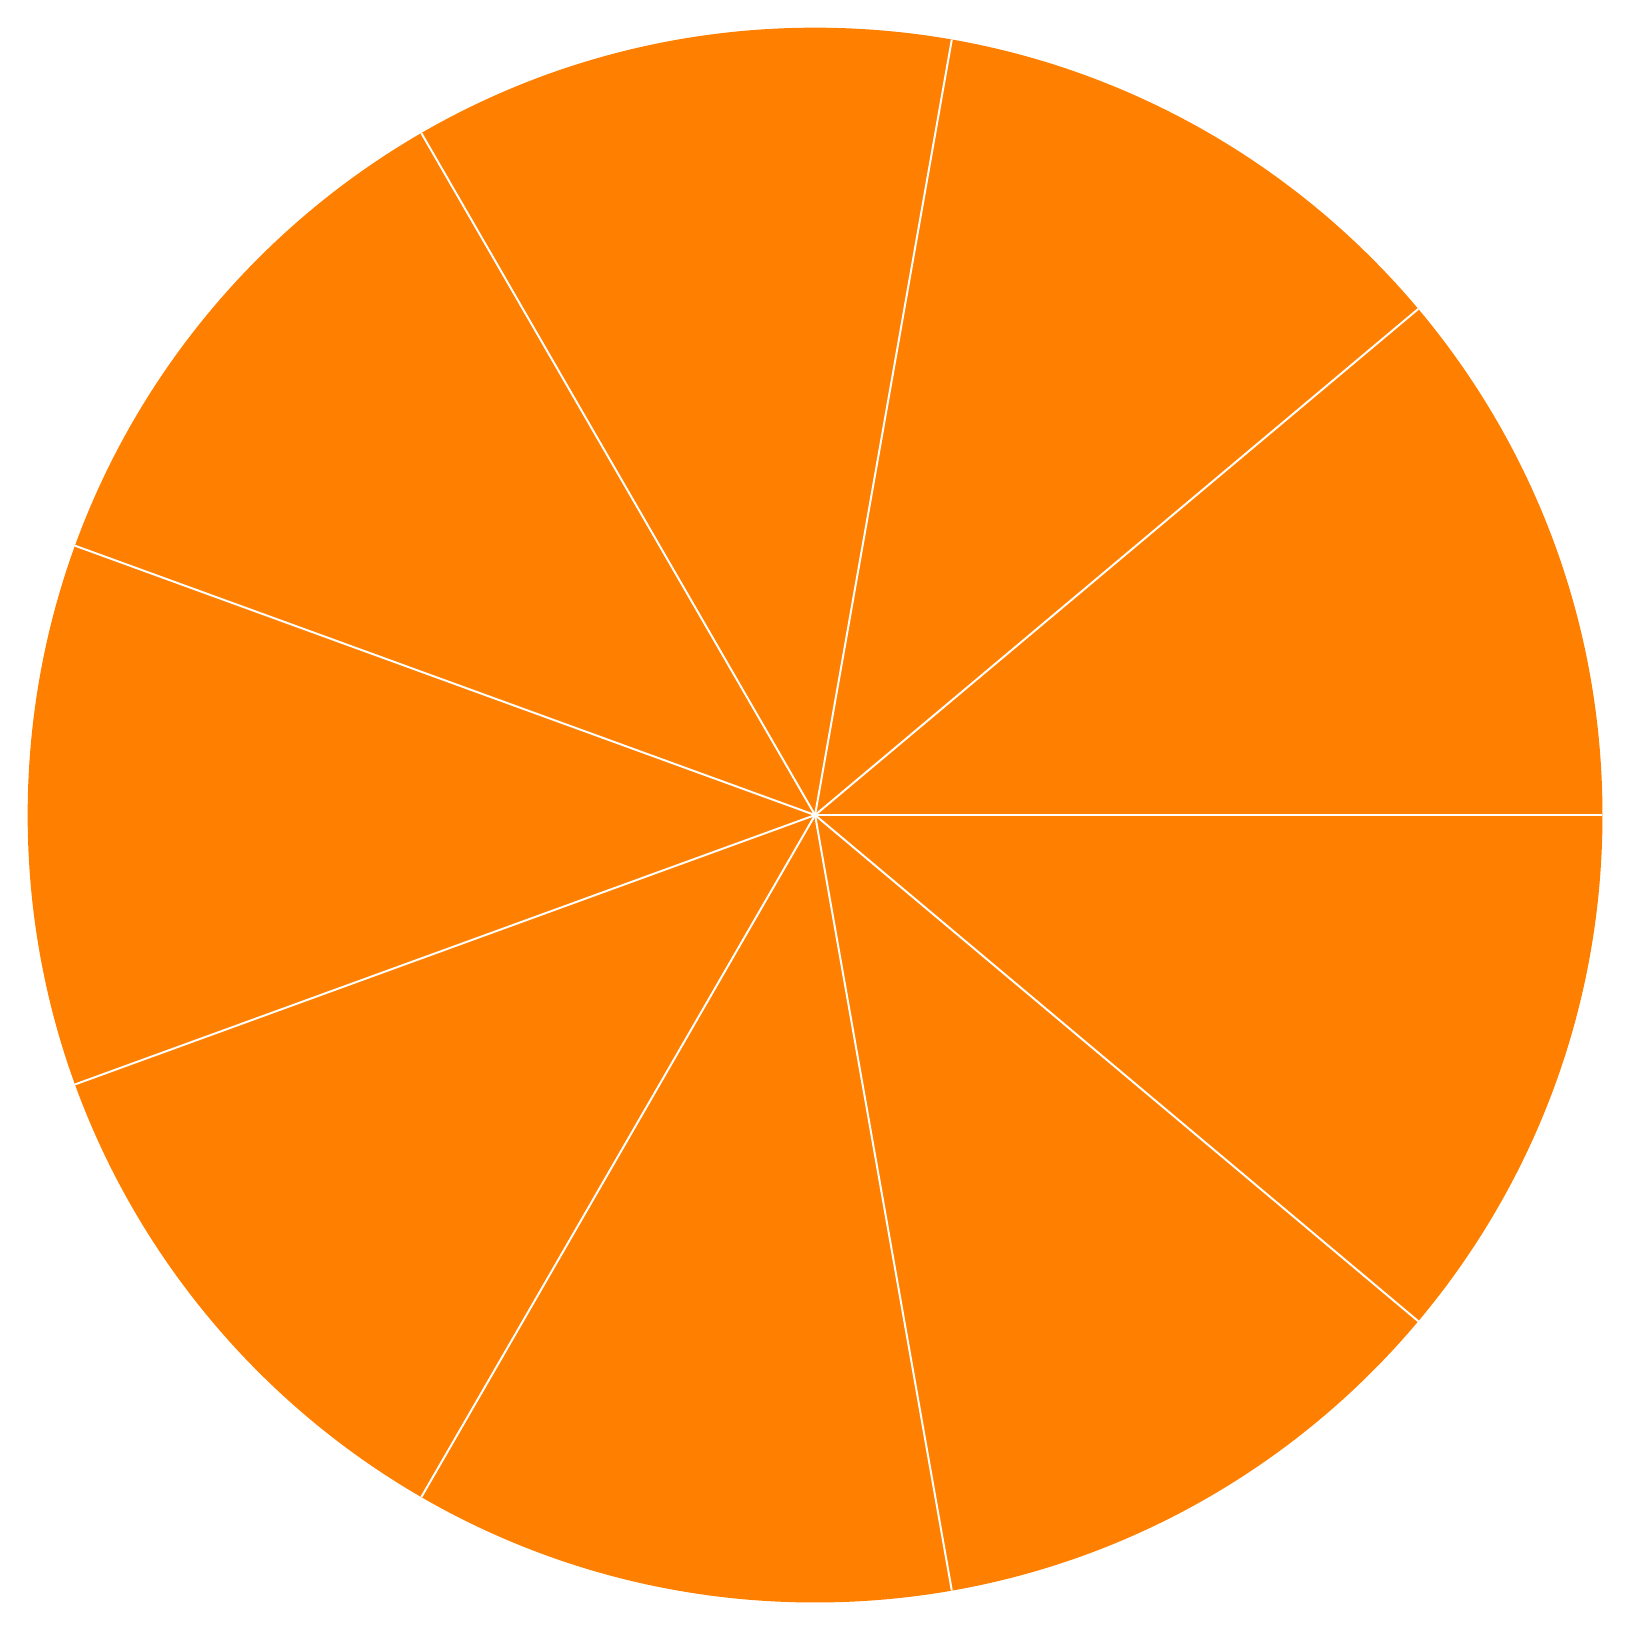
\begin{tikzpicture}
\fill[orange] (0,0) circle (10);
\foreach \x in {0,40,...,360} \draw[line width =.25mm, white] (0,0)--(\x:10);
\end{tikzpicture}
& \quad&
\begin{tikzpicture}
\draw (0,0) circle (10);
\foreach \x in {0,36,...,360} \draw[line width =.25mm] (0,0)--(\x:10);
\end{tikzpicture}

\end{tabular}

\end{center}

\begin{enumerate}[label=\alph*)]
   \item  Qual é a cor de uma peça que é um terço do círculo preto?
  \item  Qual é a cor  de uma peça que é  um quarto do círculo preto?
  \item  Qual é  a cor de uma peça que é um sétimo do círculo preto?
  \item  Qual é a cor de uma peça que é  um nono do círculo preto?
  \item  Que fração do círculo preto é uma peça de cor roxa?
  \item  Que fração do círculo preto é uma peça de cor cinza?
  \item  Que fração do círculo preto é uma peça de cor branca?
  \item  Que fração do círculo preto é uma peça de cor rosa?
  \item  Qual fração do círculo preto é maior, um terço ou um sétimo? Explique a sua resposta.
  \item  Qual fração do círculo preto é menor, um nono ou um quarto? Explique a sua resposta.
  \item  Qual fração do círculo preto é menor, um quinto ou um sétimo? Explique a sua resposta.
  \item  Qual fração do círculo preto é maior, um oitavo ou um quarto? Explique a sua resposta.
  \item  Qual fração do círculo preto é maior, um sexto ou um sétimo? Explique a sua resposta.
\end{enumerate}

\ifdefined\prof

\begin{solucao}

\begin{enumerate}[label=\alph*)]
 \item Uma peça da cor AZUL é igual a um terço do círculo preto.
 \item    Uma peça da cor VERMELHA é igual a um quarto do círculo preto.
 \item    Uma peça da cor AMARELA é igual a um sétimo do círculo preto.
 \item    Uma peça da cor LARANJA é igual a um nono do círculo preto.
 \item    Uma peça da cor roxa é igual a UM SEXTO do círculo preto.
 \item    Uma peça da cor cinza é igual a UM OITAVO do círculo preto.
 \item    Uma peça da cor branca é igual a UM DÉCIMO do círculo preto.
 \item    Uma peça da cor rosa é igual à METADE do círculo preto.
 \item    Um terço do círculo preto é maior do que um sétimo do círculo preto.
 \item    Um nono do círculo preto é menor do que um quarto do círculo preto.
 \item    Um sétimo do círculo preto é menor do que um quinto do círculo preto.
 \item    Um quarto do círculo preto é maior do que um oitavo do círculo preto.
 \item    Um sexto do círculo preto é maior do que um sétimo do círculo preto
\end{enumerate}

\end{solucao}
\fi

\end{document}